%\documentclass[twocolumn, 10pt, conference, letterpaper]{article}
\documentclass[10pt, conference, letterpaper]{IEEEtran}
%\documentclass[letterpaper, 10 pt, conference]{IEEEtran}

\usepackage[utf8]{inputenc}
\usepackage[brazilian]{babel}

%para organizar os arquivos
\usepackage{import}
\usepackage{dblfloatfix}
\usepackage{subcaption}

%para definir as margens
\usepackage{geometry}
 \geometry{
 a4paper,
 total={170mm,257mm},
 left=20mm,
 top=20mm,
 }

\usepackage{cite}
\usepackage{amsmath,amssymb,amsfonts}
\usepackage{algorithmic}
\usepackage{graphicx}
\usepackage{textcomp}
\usepackage{xcolor}
\usepackage{float}    % Melhoria de posicionamento de figuras e tabelas
\usepackage{caption}  % Personalização das legendas
%para exibir os códigos
\usepackage{minted}
\setminted{breaklines=true}
\usepackage{hyperref}

%para usar a cor de fundo
\usepackage{xcolor}
\definecolor{LightGray}{gray}{0.9}

%para imagens
\usepackage{graphicx}
\usepackage{caption}

%para inserir códigos
\usepackage{xcolor}
\definecolor{LightGray}{gray}{0.9}

%para colocar duas colunas 
\usepackage{multicol}

%para referenciar links
\usepackage{url}
  % Comment this line out if you need a4paper
\usepackage{graphicx}
\usepackage{siunitx}
\usepackage{amsmath}
\usepackage[ruled,vlined]{algorithm2e}
\usepackage{subcaption}
%\documentclass[letterpaper, 10 pt, conference]{ieeeconf}
\title{Efeitos da variação da taxa de compressão sobre a eficiência do Ciclo de Otto para motores de combustão interna

\author{\IEEEauthorblockN{Victor Matteus S. Souza}
\textit{Matrícula: 202105201} \\
\IEEEauthorblockA{\textit{Instituto de Física(IF)} \\
\textit{UFG}\\
Goiânia, Goiás}
\and
\IEEEauthorblockN{Guilherme Vinícius B. de A. Vieira}
\textit{Matrícula: 202105589} \\
\IEEEauthorblockA{\textit{Instituto de Física(IF)} \\
\textit{UFG}\\
Goiânia, Goiás}
\and

\IEEEauthorblockN{Diogo Pereira Nascimento}
\textit{Matrícula: 202105179} \\
\IEEEauthorblockA{\textit{Instituto de Física(IF)} \\
\textit{UFG}\\
Goiânia, Goiás}
}

}
\begin{document}
\maketitle
\thispagestyle{empty}
\pagestyle{empty}
\begin{abstract}
Este estudo de física computacional investiga a eficiência do ciclo termodinâmico de Otto em motores de combustão interna, considerando variações nas taxas de compressão. Um código em Python foi desenvolvido para analisar e gerar gráficos relacionados ao desempenho e eficiência do ciclo. O estudo busca compreender o impacto de diferentes valores de taxa de compressão no desempenho de um cilindro operante, explorando parâmetros como trabalho por ciclo e potência gerada.
\end{abstract}

\section{Introdução}
%AQUI COMECE COM UMA DESCRIÇÃO DE TEORIA TERMODINÂMICA, MÁQUINAS TÉRMICAS E IMPORTÂNCIA DELAS, APRESENTANDO O CICLO DE OTTO NO FINAL
\hspace{0.5cm}O século XIX marcou a história da humanidade com a Segunda Revolução Industrial, que teve como um dos grandes passos tecnológicos o desenvolvimento do motor a combustão. Todo esse avanço teve como base os estudos na termodinâmica.

\hspace{0.5cm}A termodinâmica é o ramo da física que estuda as relações entre energia, calor, trabalho e as propriedades das substância, que tem como objetivo descrever os processos físicos e químicos que envolvem a transferência de energia na forma de calor e trabalho, bem como as mudanças de estado de substâncias. Uma série de processos termodinâmicos que levam o sistema de volta ao seu estado inicial pode ser definido como um ciclo termodinâmico.

\hspace{0.5cm}Dito isso, tem-se que motores de combustão interna são máquinas térmicas que transformam a energia proveniente de uma reação química em energia mecânica. Esse processo de conversão é feito através de ciclos termodinâmicos que envolvem a compressão e expansão de gases gerando uma mudança de temperatura neles \cite{reference5}. Dentre tais motores, há, então, aqueles que se utilizam do Ciclo Termodinâmico de Otto como base de seu funcionamento.


\subsection{Descrição Histórica do Otto}
% AQUI FALE UM POUCO DA HISTÓRIA DO CICLO DE OTTO E IMPLICAÇÕES, APLICAÇÕES E IMPORTÂNCIA DELE NOS DIAS DE HOJE;

\hspace{0.5cm}Alphonse Beau de Rochas foi um engenheiro francês que, em 1862, idealizou o ciclo fechado termodinâmico em que se alternavam duas evoluções adiabáticas e outras duas isocóricas. No entanto, apesar do engenheiro francês ter sido o primeiro a desenvolver esse ciclo, os estudos desenvolvidos pelos alemães Nikolaus August Otto, Gottlieb Daimler e Wilhelm Maybach, acabaram se tornando os mais relevantes na área, por conseguirem desenvolver um motor prático de alta eficiência, desempenho e potência.

\hspace{0.5cm}Os trabalhos de Otto foram feitos de forma independente ao de Beau de Rochas e tiveram sua conclusão em 1876, na construção do primeiro motor que utilizaria o Ciclo de Otto. Nos anos seguintes, outros engenheiros utilizaram das ideias de Otto para confecção de seus próprios motores, como o motor Daimler, por exemplo, que foi de extrema importância para o desenvolvimento do automobilismo.

\hspace{0.5cm}Hoje em dia, o Ciclo de Otto é amplamente utilizado nas indústrias e em automóveis, utilizando combustíveis leves como gasolina, álcool ou gás natural \cite{reference2}.
	
\subsection{Descrição Teórica}\label{intro:des-teorica}

\hspace{0.5cm}O ciclo de Otto possui quatro curvas termodinâmicas que descrevem o comportamento do sistema como um todo. O ciclo é formado por duas etapas isovolumétricas com variação da quantidade de calor (combustão e escape) e por duas isentrópicas, em que a pressão e o volume variam (admissão e compressão), 
 como demonstrado na Figura. \ref{fig:motor-ilustracao}. 

\begin{figure}[H]
    \centering
    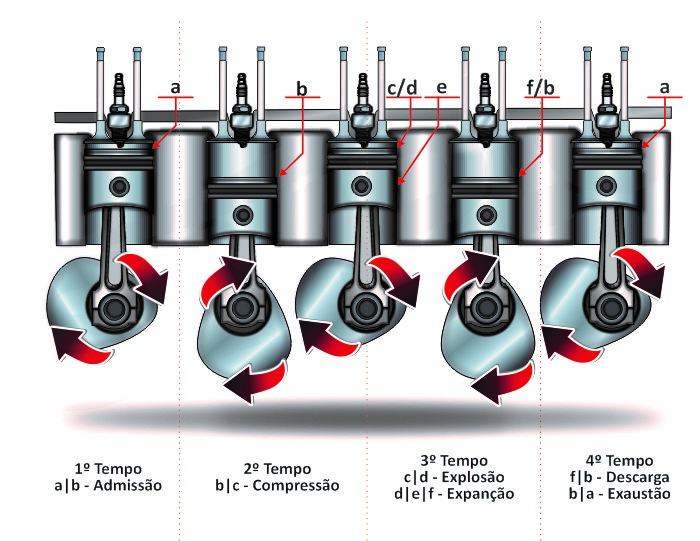
\includegraphics[width=\columnwidth]{Imagens/etapas-do-motor-ciclo-otto.jpg}
    \caption{Ilustração das etapas de admissão, compressão, combustão e exaustão de um motor termodinâmico que opera em ciclos. Retirada de \cite{reference3}.}
    \label{fig:motor-ilustracao}
\end{figure}

%\hspace{0.5cm} Tal como ilustrado pela Figura \ref{fig:motor-ilustracao}, que traz as etapas do ciclo
As etapas, como já citadas anteriormente, são dividas da seguinte forma:
\begin{enumerate}
    \item \textbf{Admissão:} Durante esta fase, uma mistura de ar e combustível é admitida na câmara de combustão através da abertura da válvula de admissão. Aumenta-se o volume da câmara, mantendo a pressão baixa.
    
    \item \textbf{Compressão:} A válvula de admissão é fechada e o pistão comprime a mistura ar-combustível. Isso aumenta significativamente a pressão e a temperatura da mistura. A compressão ocorre de forma adiabática.
        
    \item \textbf{Combustão:} Após a compressão, uma vela de ignição causa a ignição da mistura ar-combustível. A queima rápida e controlada leva a um aumento rápido na pressão, empurrando o pistão para baixo.
        
    \item \textbf{Escape:} A válvula de escape é aberta e os gases resultantes da queima são expelidos da câmara de combustão à medida que o pistão retorna à posição superior. Isso completa um ciclo e prepara o motor para o próximo ciclo.
\end{enumerate}

\subsection{Eficiência do Ciclo de Otto}

\hspace{0.5cm}A eficiência no ciclo de Otto é descrita a partir de uma análise matemática da energia interna, do calor e do trabalho em cada tempo do motor. A Figura \ref{fig:etapas-otto-grafico} mostra como funciona uma máquina ideal em relação a pressão em função do volume dentro do sistema.

\begin{itemize}
    \item Para os processos adiabáticos (curvas \textbf{1-2} e \textbf{3-4}):
    \begin{equation}\label{1}
    \frac{W_{\text{12}}}{m}=(u_{\text{2}}-u_{\text{1}})
    \end{equation}
    \begin{equation}\label{2}
    \frac{W_{\text{34}}}{m}=(u_{\text{3}}-u_{\text{4}})
    \end{equation}
    Associando ambas as equações pode-se dizer:
    \begin{equation}\label{3}
    \frac{W_{\text{ciclo}}}{m}=\frac{W_{\text{34}}}{m}-\frac{W_{\text{12}}}{m}=(u_{\text{3}}-u_{\text{4}})-(u_{\text{2}}-u_{\text{1}})
    \end{equation}

    \item Para os processos isovolumétricos (curvas \textbf{2-3} e \textbf{4-1}):
    \begin{equation}\label{4}
    \frac{Q_{\text{23}}}{m}=(u_{\text{3}}-u_{\text{2}})
    \end{equation}
    \begin{equation}\label{5}
    \frac{W_{\text{41}}}{m}=(u_{\text{4}}-u_{\text{1}})
    \end{equation}
    Associando os modelos:
    \begin{equation}\label{6}
    \frac{Q_{\text{ciclo}}}{m}=\frac{Q_{\text{23}}}{m}-\frac{Q_{\text{41}}}{m}=(u_{\text{3}}-u_{\text{2}})-(u_{\text{4}}-u_{\text{1}})
    \end{equation}
\end{itemize}

\begin{figure}[!ht]
    \centering
    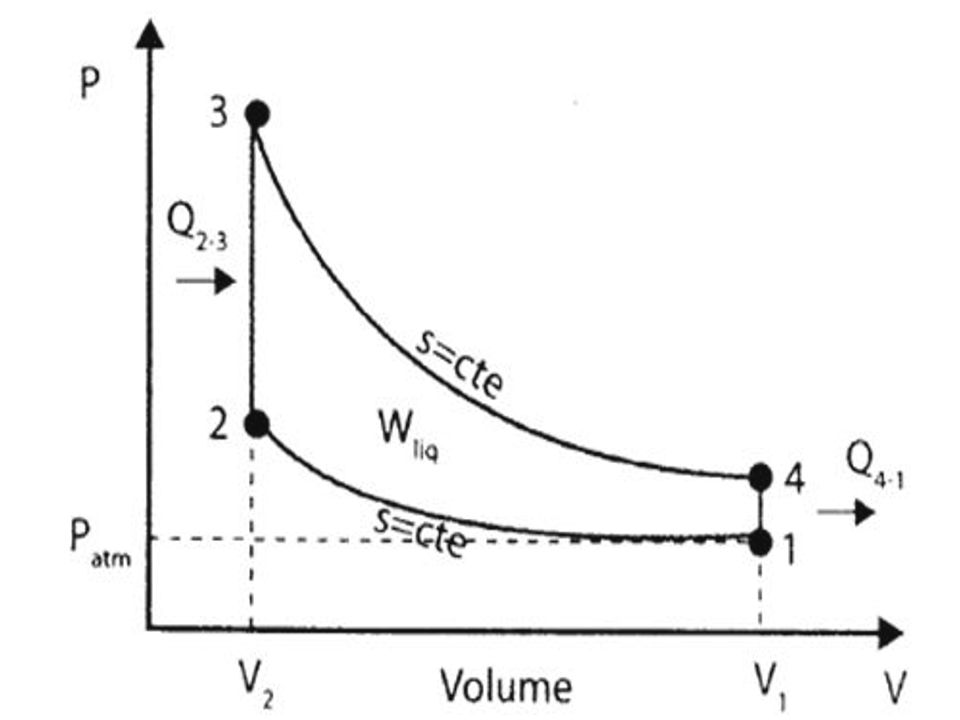
\includegraphics[width=\columnwidth]{Imagens/CIcloOttoPV.jpg}
    \caption{Etapas do ciclo de Otto. Os caminhos \textbf{4-1} e \textbf{2-3} possuem comportamento isovolumétrico na qual são referentes aos processos de combustão e de escape enquanto os tempos \textbf{1-2} e \textbf{3-4} possuem variações de pressão e volume sendo esses, respectivamente, os processos de compressão e admissão. Figura retirada de \cite{reference1}. }
    \label{fig:etapas-otto-grafico}
\end{figure}


A eficiência térmica de uma máquina é descrita como a razão do calor do ciclo pelo trabalho realizado. Com base nesse conhecimento e nas equações já desenvolvidas, pode-se afirmar que a eficiência é dada por:
    \begin{equation}\label{7}
    \eta=\frac{(u_{\text{3}}-u_{\text{4}})-(u_{\text{2}}-u_{\text{1}})}{(u_{\text{3}}-u_{\text{2}})-(u_{\text{4}}-u_{\text{1}})}=1-\frac{(u_{\text{4}}-u_{\text{1}})}{(u_{\text{3}}-u_{\text{2}})}
    \end{equation}
    Onde fundamentalmente\cite{reference1} sabemos que: 
    \begin{equation}\label{8}
    \Delta u=c_{\text{v}}(T_{\text{a}}-T_{\text{b}})
    \end{equation}

Assim, substituindo a equação \ref{8} na equação \ref{7}, obtém-se:
\begin{equation}\label{9}
\eta=1-\frac{c_{\text{v}}(T_{\text{4}}-T_{\text{1}})}{c_{\text{v}}(T_{\text{3}}-T_{\text{2}})}=1-\frac{T_{\text{1}}}{T_{\text{2}}}
\end{equation}

Utilizando outra relação termodinâmica:
\begin{equation}\label{10}
\frac{T_{\text{2}}}{T_{\text{1}}}=(\frac{V_{\text{1}}}{V_{\text{2}}})^{\gamma-1}=C_r^{\gamma-1}
\end{equation}

Na qual a variável $C_r$ designa a taxa de compressão do sistema e $\gamma$ é a razão entre o calor específico para pressão constante e o calor específico para volume constante. A partir dessa equação \ref{10}, é possível chegar à seguinte expressão para a eficiência térmica do motor:

\begin{equation}\label{11}
    \eta = 1 - \frac{1}{C_r^{\gamma - 1}}
\end{equation}\newline

Conclui-se, portanto, que quanto maior a taxa de compressão $C_r$, maior será o rendimento do motor.

\subsection{Características Físicas do Sistema}\label{intro:características-do-sistema}

Na análise do sistema, pode-se descrever as variáveis termodinâmicas como o volume e a pressão em função de termos que descrevem de forma cinemática o funcionamento de uma válvula de um motor.
\newline
\begin{itemize}

    \item \textbf{Cilindrada:} é o volume máximo da mistura de ar e combustível admitido dentro do pistão em um ciclo, que dá a informação da quantidade de combustível e/ou ar aspirado e retirado do motor. Pode ser definido matematicamente como: 
    \begin{equation}
    V_s=\frac{\pi}{4}d^2L\label{12}    
    \end{equation}
    Sendo $V_s$ a cilindrada, d o diâmetro do cilindro e L a altura do diâmetro.\newline

    \item \textbf{Volume morto ou volume de folga:} informa quanto volume original foi compactado; também pode ser definido como a diferença entre o volume total do cilindro e cilindrada. O espaço coberto pelo volume morto também forma a câmara de combustão. Pode ser definido matematicamente como:
    \begin{equation}
    V_c= V_t-V_s\label{13}
    \end{equation}
    Sendo $V_c$ o volume morto e $V_t$ o volume total.\newline

    \item \textbf{Taxa de compressão:} pode ser definido como o valor obtido após dividir o volume total do cilindro pelo volume morto.
    \begin{equation}
    C_r=\frac{V_t}{V_c}\label{14}
    \end{equation}
    Sendo $C_r$ a taxa de compressão.\newline

    Usando o conceito de taxa de compressão, é possível definir o volume morto como:
    \begin{equation}
    V_c=\frac{V_s}{C_r-1}\label{15}
    \end{equation}

    \item \textbf{Volume do cilindro do pistão:} pode ser determinado em função do ângulo da manivela a partir da taxa de compressão, do curso, do diâmetro interno e do comprimento da biela. 
    \begin{equation}
    V=\frac{V_s}{C_r-1}+\frac{V_s}{2}[1+R-cos(\theta)-\sqrt{R^2-sen(\theta)}]\label{16}
    \end{equation}
    Sendo V o volume do cilindro do pistão e R a metade do comprimento da biela.

\end{itemize}

\begin{figure}[H]
    \centering
    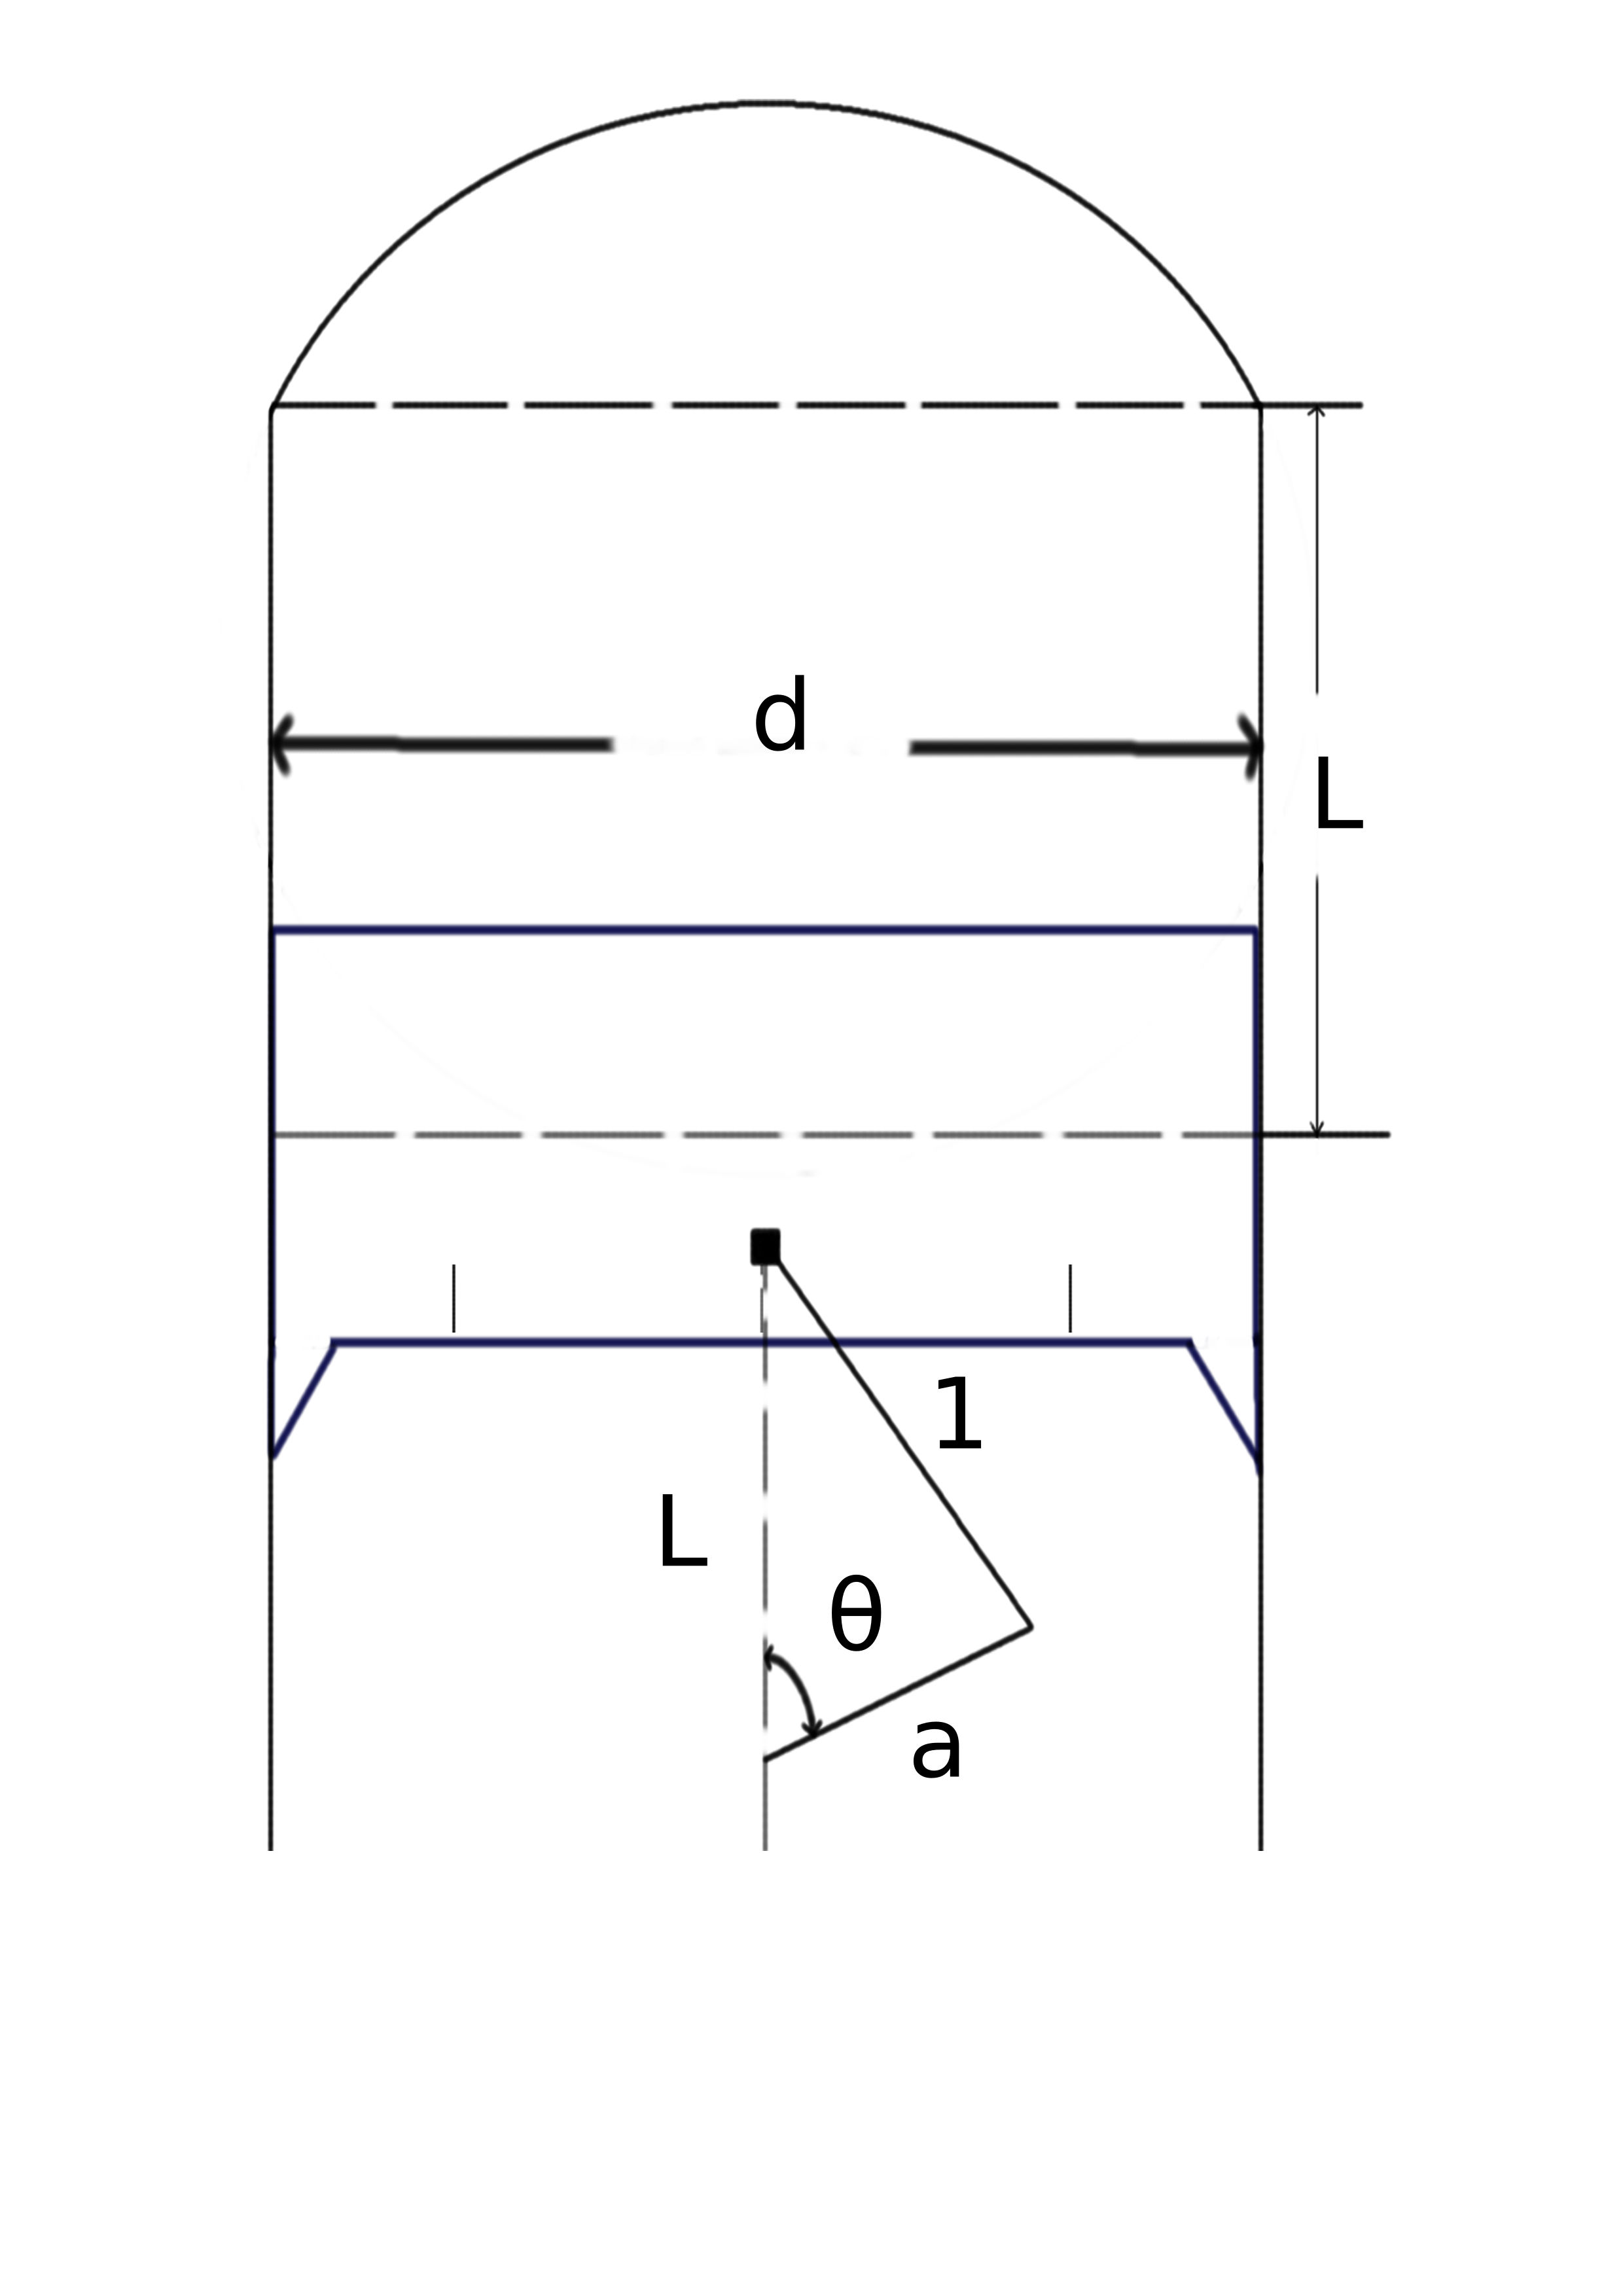
\includegraphics[width=\columnwidth]{Imagens/cilindro1.jpg}
    \caption{Esquema de uma válvula cilíndrica.}
    \label{fig:imagem-do-cilindro}
\end{figure}

\section{Objetivos}
Assim sendo, tem-se que este artigo tem por objetivo investigar, avaliar e encontrar computacionalmente a eficiência do ciclo termodinâmico de Otto em motores de combustão interna, considerando variações das taxas de compressão $C_r$. Para isso, buscamos compreender como diferentes valores de $C_r$ afetam o desempenho e a eficiência de um cilindro operante, analisando parâmetros como o trabalho por ciclo e a potência gerada e gráficos gerados do ciclo. \newline

\section{Metodologia}
Conforme dito anteriormente, a eficiência ($\eta$) de um ciclo termodinâmico depende diretamente das variáveis de estado e das relações entre elas no decorrer de seus processos. Tal fato torna possível então o cálculo de seu valor por meio da equação \ref{11}, que relaciona $\eta$ a taxa de compressão ($C_r$), que por sua vez depende das variávies de estado V e T, conforme equação \ref{10}. 

Assim sendo, o \textit{script python} desenvolvido é iniciado com a importação das bibliotecas necessárias e da adquirição, por meio de entradas do usuário, das variáveis que definem as propriedades geométricas do cilindro como pode-se observar na figura \ref{fig:imagem-do-cilindro}. Tais passos podem ser encontrados nos Apêndices \ref{apend:bibliotecas} e \ref{apend:entradas}.

A seguir, como mostrado no apêndice \ref{apend:cinematica-pistao}, é definida a função "cinemática do pistão", que recebe como parâmetros as características geométricas do cilindro, a taxa de compressão e os ângulos $\theta$ do início e final do processo, como explicado na seção \ref{intro:características-do-sistema}. A função calcula primeiramente os volumes de deslocamento e folga das equações \ref{12} e \ref{15}. Após isso, dentro de um processo iterativo, calcula a variação angular do ângulo $\theta$ para determinar volume do pistão, que é então adicionado a uma lista. Essa lista é então retornada como resultado da função.

Uma vez apresentada a função que retorna o volume ocupado dentro do cilindro, pode-se iniciar o cálculo das variáveis de estado em cada etapa do ciclo. Assim como explicado na seção \ref{intro:des-teorica}, o ciclo operante de um motor de combustão interna é composto de 4 etapas básicas: admissão, compressão, ignição e exaustão. Tais etapas se traduzem no Ciclo de Otto também em 4 estados, sendo eles: compressão, adição de calor, expansão e rejeição de calor. Desta forma, para obter a ilustração desse processo em um diagrama $P$x$V$ (pressão \textit{versus} volume), é necessário realizar o cálculo das variáveis de estado P, V e T em cada instante desse processo. O Apêndice \ref{apend:estados-ciclo} é o trecho de código responsável por esses cálculos. Para tal, tem-se que foram utilizadas as equações \ref{10}, \ref{12}, \ref{13} e \ref{15}, além da função de cinemática do pistão e da equação geral de transformação dos gases, definida por: 

\begin{figure*}[!ht]
    \centering
    
    \begin{subfigure}{0.45\textwidth}
        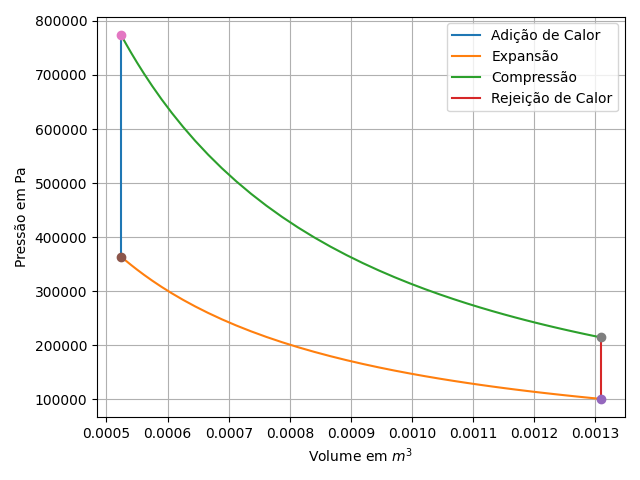
\includegraphics[width=\linewidth]{Imagens/grafico_cr25.png}
        \caption{Ciclo de Otto para \(C_r  = 2.5\) }
        \label{fig:cr25}
    \end{subfigure}
    \hfill
    \begin{subfigure}{0.45\textwidth}
        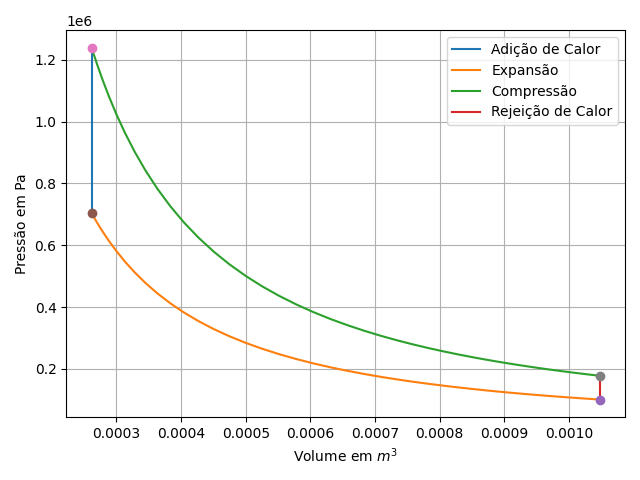
\includegraphics[width=\linewidth]{Imagens/grafico_cr40.png}
        \caption{Ciclo de Otto para \(C_r  = 4.0\) }
        \label{fig:cr40}
    \end{subfigure}
    
    \begin{subfigure}{0.45\textwidth}
        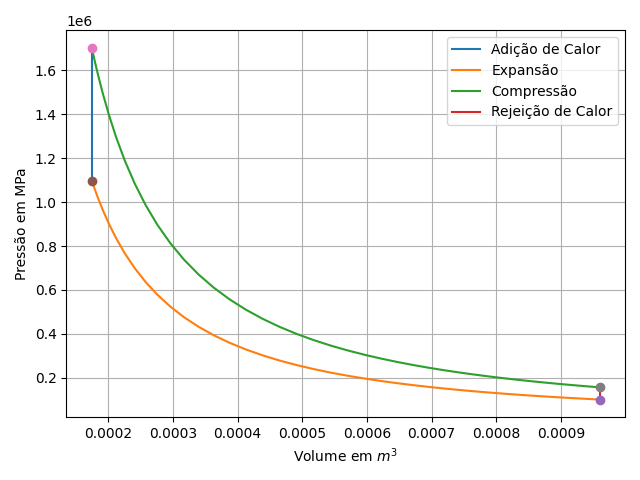
\includegraphics[width=\linewidth]{Imagens/grafico_cr55.png}
        \caption{Ciclo de Otto para \(C_r  = 5.5\) }
        \label{fig:cr55}
    \end{subfigure}
    \hfill
    \begin{subfigure}{0.45\textwidth}
        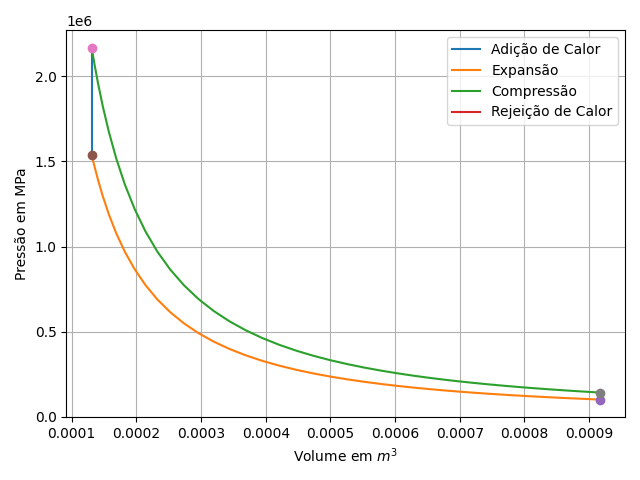
\includegraphics[width=\linewidth]{Imagens/grafico_cr70.png}
        \caption{Ciclo de Otto para \(C_r  = 7.0\) }
        \label{fig:cr70}
    \end{subfigure}
    
    \caption{Ciclos de Otto para diferentes valores de Taxa de Compressão (Cr) para isotermas $T_1 = 750K$ e $T_2 = 2300K$ para um cilindro de  $0.0015 cm^3$ . Note que o ciclo ocorre no sentido horário, passando pelas fases de compressão, adição de calor, expansão e rejeição de calor.}
    \label{fig:ciclos_otto}
\end{figure*}

\begin{table*}[hb]%se você qur forçar a posição dela exatamente aqui onde você colocou e não onde o programa achar melhor, vc coloca um H (maiúsculo) no lugar do hb
\centering
\caption{Resultados obtidos para o trabalho, potência e eficiência para cada Ciclo de Otto de um cilindro de  $0.0015 cm^3$  da figura \ref{fig:ciclos_otto}.}
\label{tab:my-table}
\begin{tabular}{|c|c|c|c|c|c|}
\hline
\multicolumn{1}{|c|}{\begin{tabular}[c]{@{}c@{}}Taxa de \\ Compressão(Cr)\end{tabular}} & \begin{tabular}[c]{@{}c@{}}Trabalho\\ Expansão(J)\end{tabular} & \begin{tabular}[c]{@{}c@{}}Trabalho \\ Compressão(J)\end{tabular} & \begin{tabular}[c]{@{}c@{}}Trabalho Total \\ por Ciclo(J)\end{tabular} & \begin{tabular}[c]{@{}c@{}}Potência a\\ 3000 rpm (kW)\end{tabular} & Eficiência(\%) \\ \hline
2,5                                                                                   & 608,16                                                                             & -79,33                                                                                & 528,83                                                                                     & 26,44                                                                                  & 39,69                           \\ \hline
4,0                                                                                     & 973,06                                                                             & -79,33                                                                                & 893,73                                                                                     & 44,69                                                                                 & 42,57                            \\ \hline
5,5                                                                                   & 1337,95                                                                             & -79,33                                                                                & 1258,63                                                                                      & 62,93                                                                                 & 49,53                            \\ \hline
7,0                                                                                     & 1702,85                                                                             & -79,33                                                                                & 1623,52                                                                                     & 81,18                                                                                 & 54,08                            \\ \hline
\end{tabular}
\end{table*}

\begin{equation}
    \frac{P_1V_1}{T_1} = \frac{P_2V_2}{T_2}\label{17}
\end{equation}

Uma vez de posse das variáveis de estado, pode-se então realizar os cálculos energéticos do sistema, conforme o trecho de código do Apêndice \ref{apend:efic-trab-pot}. Tal trecho define primeiramente uma função que realiza o cálculo do trabalho gasto por etapa do ciclo, recebendo como parâmetros as variáveis de estado pressão e volume e retornando o trabalho em cada estado e o trabalho por ciclo. Para o cálculo da potência, defini-se primeiramente um parâmetro comparativo de revoluções por minuto do cilindro, de forma a simular o que ocorre em um motor real. Dessa forma, a potência será dada por:

\begin{equation}
    Pot = \frac{W_{ciclo}r_pm}{60}
\end{equation}

Por fim, é possível realizar a plotagem do gráfico que representa o Ciclo de Otto para o cilindro em questão, além de realizar a impressão dos resultados obtidos no decorrer da execução do código. Isso está explicito nos Apêndices \ref{apend:resultados} e \ref{apend:plot-graficos}. 

\section{Resultados e Discussões}
Para o teste do código bem como explicação dos fenômenos físicos envolvidos que interferem na eficiência do ciclo, foram realizados 4 testes à pressão inicial de $101kPa$ e à temperaturas entre $750K$ e $2300K$ para um cilindro de $0.1 m$ diâmetro, $0.1 m$ de curso e $0.15 m$ de biela. Para cada teste, o parâmetro taxa de compressão ($C_r$) foi alterado com o intuito de se observar as modificações no gráfico $P$x$V$ do ciclo, bem como de seus respectivos valores energéticos. Tais resultados podem ser observados através da figura \ref{fig:ciclos_otto} e da tabela \ref{tab:my-table}.

Nota-se, a princípio, que  quanto maior a taxa de compressão ($C_r$) inserida pela usuário, maior é a eficiência $\eta$ do ciclo. Tal resultado confirma em termos práticos a veracidade da equação de rendimento equação \ref{11}. 

Além disso, percebe-se também que o trabalho gerado por ciclo também aumenta com o coeficiente $C_r$, e, consequentemente, o mesmo ocorre para a potência. Isso ocorre devido ao fato de que seu aumento acarreta o aumento da razão de expansão (equação \ref{14}), o que significa uma maior variação de volume durante o ciclo na fase de expansão, gerando maior trabalho de expansão. Dessa forma, o trabalho líquido total por ciclo é também maior.



\section{Conclusão}
Por fim, conclui-se que a taxa de compressão $C_r$ é um parâmetro importante em motores de combustão interna, como o ciclo de quatro tempos do motor Otto. Isso se deve dado que essa taxa afeta a eficiência e o desempenho do motor de várias maneiras, como pôde-se observar nos gráficos. Assim, ocorre o aumento do trabalho realizado pelo motor quando a taxa de compressão é aumentada. Sobretudo, têm-se que sua variação acarreta efeitos claros sobre a eficiência termodinâmica e a razão de expansão do motor, conforme demonstradas nesse artigo. 

%\newpage
%============================================================================
%============================================================================
%APÊNDICES
%============================================================================
%============================================================================

\section{Apêndices}
    \subsection{Bibliotecas}\label{apend:bibliotecas}
        Trecho responsável por fazer a importação das bibliotecas a serem utilizadas ao longo do código.
        \inputminted[
        frame=lines,
        framesep=2mm,
        baselinestretch=1.2,
        bgcolor=LightGray,
        fontsize=\scriptsize,
        ]{python}{scripts/bibliotecas.py}

    \subsection{Entradas}\label{apend:entradas}
        Trecho do código responsável por adquirir do usuário as características geométricas do cilindro a ser avalidado. Além disso, define-se o calor específico do ar \(\gamma = 1.4\) e a taxa de compressão. 
        \inputminted[
        frame=lines,
        framesep=2mm,
        baselinestretch=1.2,
        bgcolor=LightGray,
        fontsize=\scriptsize,
        ]{python}{scripts/entradas.py}
    
    \subsection{Cinemática do Pistão}\label{apend:cinematica-pistao}
        Trecho de código responsável que descreve a função "cinemática-pistão". Tal função recebe como parâmetros o diâmetro, curso, biela, taxa de compressão, ângulo-inicial e ângulo-final do pistão e calcula os volumes de folga e deslocamento do pistão.
        \inputminted[
        frame=lines,
        framesep=2mm,
        baselinestretch=1.2,
        bgcolor=LightGray,
        fontsize=\scriptsize,
        ]{python}{scripts/cinematica_pistao.py}   
        
    \subsection{Estados do Ciclo}\label{apend:estados-ciclo}
        Trecho do código responsável por calcular os valores de pressão, temperatura e volume para o ciclo.
        \inputminted[
        frame=lines,
        framesep=2mm,
        baselinestretch=1.2,
        bgcolor=LightGray,
        fontsize=\scriptsize,
        ]{python}{scripts/estados_do_ciclo.py} 
        
    \subsection{Cálculo da eficiência, trabalho e potência}\label{apend:efic-trab-pot}
        Trecho do código responsável por realizar o cálculo do trabalho em cada estado por meio da definição da função "calcular-trabalho". Além disso, calcula a eficiência e a potência gerada pelo cilindro a uma certa quantidade de revoluções por minuto.
        \inputminted[
        frame=lines,
        framesep=2mm,
        baselinestretch=1.2,
        bgcolor=LightGray,
        fontsize=\scriptsize,
        ]{python}{scripts/eficiencia_energia.py}    
        
    \subsection{Impressão dos resultados}\label{apend:resultados}
        Trecho do código responsável por imprimir os resultados de trabalho, eficiência e potência calculados. Além disso, armazena os 4 valores principais de pressão, volume e temperatura presentes no gráfico gerado.
        \inputminted[
        frame=lines,
        framesep=2mm,
        baselinestretch=1.2,
        bgcolor=LightGray,
        fontsize=\scriptsize,
        ]{python}{scripts/impressao_resultados.py}  
        
    \subsection{Plotagem de Gráficos}\label{apend:plot-graficos}
        Trecho responsável por plotar o gráfico \(PxV\) do ciclo de Otto, atendando-se para os quatro pontos de mudança de curva para determinado coeficiente taxa de compressão (Cr).
        \inputminted[
        frame=lines,
        framesep=2mm,
        baselinestretch=1.2,
        bgcolor=LightGray,
        fontsize=\scriptsize,
        ]{python}{scripts/plotagem_grafico.py}  
        
    \subsection{Apresentação em vídeo}
        Segue o link do vídeo de apresentação requerido para o trabalho:
        \begin{itemize}
            \item \url{https://youtu.be/vKrciZkwJuI}
        \end{itemize}

    \subsection{Código}
        Segue o link do código disponibilizado no Google Colaboratory:
        \begin{itemize}
            \item \url{https://colab.research.google.com/drive/1iNzoSAbDizIpOeDhHVLPJPpRXgoMYnXJ?usp=sharing}
        \end{itemize}
    
%============================================================================
%============================================================================
%============================================================================
%============================================================================

%\section{Referências Bibliográficas}
\bibliographystyle{plain}
\bibliography{sample}

\end{document}


